
\chapter{Fourier Transform of a vector valued distribution}\label{chap8}


One\pageoriginale knows (Theorie des distributions, tome~2, \S~6, Chap.~VII) that
the Fourier transform $\mathscr{F}$ is a topological isomorphism of
$\mathscr{S}'$ on $\mathscr{S}'$, and the inverse of $\mathscr{F}$
which is also a topological isomorphism is called the conjugate of
$\mathscr{F}$ and is denoted by $\mathscr{\bar{F}}$.

\setcounter{section}{8}
\setcounter{definition}{0}
\begin{definition}\label{chap8:def8.1}
Let $E$ be a complete $E L C$. Let $I$ be the identity map of $E$. The
continuous linear map $\mathscr{F} \in I$ of $\mathscr{S}'
(E)$ in $\mathscr{S}' (E)$ is called the Fourier transform of
$\mathscr{S}'(E)$ into itself.

Using the fact that $\bar{\mathscr{F}}$ is the inverse of
$\mathscr{F}$ and that $(\mathscr{F} \in I)(\bar{\mathscr{F}}
\in I) = \mathscr{F} \bar{\mathscr{F}} \in I$ we see
that $\mathscr{F} \in I$ $\mathscr{S}'(E) \to \mathscr{S}'(E)$
is in fact an automorphism. We agree to denote the automorphism also
by $\mathscr{F}$.
\end{definition}

\setcounter{section}{8}
\setcounter{prop}{0}
\begin{prop}\label{chap8:prop8.1}
For $\overrightarrow{T} \in \mathscr{S}'(E)$ and $\varphi
\in \mathscr{S}$ we have
$$
\mathscr{F} \overrightarrow{T} (\varphi) = \overrightarrow{T}
(\mathscr{F} \varphi).
$$
\end{prop}
\begin{proof}
The Fourier transform of any $T \in \mathscr{S}'$ is defined
exactly by the equality $\mathscr{F} T (\varphi) = T (\mathscr{F}
\varphi)$, for every $\varphi \in \mathscr{S}$. To prove
$\mathscr{F} \overrightarrow{T} (\varphi)=\overrightarrow{T}
(\mathscr{F} \varphi)$ we have to only form the scalar product with
any $\overleftarrow{e}' \in E'$ and apply the equality
$\mathscr{F} T (\varphi) = T(\mathscr{F} \varphi)$, for any $T
\in \mathscr{S}', \varphi \in \mathscr{S}$. In fact,
\begin{align*}
\langle \mathscr{F} \overrightarrow{T} (\varphi),
\overleftarrow{e}'\rangle &= \langle \mathscr{F} \overrightarrow{T},
\overleftarrow{e}' \rangle (\varphi) = \mathscr{F} \langle
\overrightarrow{T}, \overleftarrow{e}'\rangle (\varphi)\\
&= \langle \overrightarrow{T}, \overleftarrow{e}' \rangle (\mathscr{F}
\varphi) = \langle \overrightarrow{T} (\mathscr{F} \varphi),
\overleftarrow{e}'\rangle.
\end{align*}
This proves $\mathscr{F} \overrightarrow{T} (\varphi) =
\overrightarrow{T} (\mathscr{F} \varphi)$.
\end{proof}

\begin{prop}\label{chap8:prop8.2}
For every $\overrightarrow{T} \in \mathscr{S}' (E)$ and $s\in
\mathscr{O}_M$ we have $\mathscr{F}
(\overrightarrow{T}\cdot s)=\mathscr{F}(\overrightarrow{T})\ast\mathscr{F} s$ where
$\overrightarrow{T}\cdot s$ denotes the multiplicative product of
$\overrightarrow{T} \in \mathscr{S}' (E)$ and $s \in\underset{M}{\mathscr{O}}$.
\end{prop}

\begin{proof}
One\pageoriginale knows (Theorie des distributions, tome 2) that the multiplicative
product $T\cdot s$ of any $T \in \mathscr{S}'$ and $s \in \mathscr{O}_M$, is
an element of $\mathscr{S}'$. Hence for any $\overrightarrow{T} \in
\mathscr{S}'(E)$ and $s \in \mathscr{O}_M, \overrightarrow{T} \cdot s \in
\mathscr{S}'(E)$. Also one knows the validity of the equality
$\mathscr{F} (T \cdot s) = \mathscr{F} (T) \ast \mathscr{F} s$ for any $T
\in \mathscr{S}'$ and $s \in \mathscr{O}_M$. Now, for any
$\overleftarrow{e}' \in E'$,
\begin{align*}
\langle \mathscr{F} (\overrightarrow{T} \cdot s), \overleftarrow{e}'\rangle
&= \mathscr{F} \langle \overrightarrow{T} \cdot s, \overleftarrow{e}'
\rangle\\
&= \mathscr{F} ( \langle \overrightarrow{T}, \overleftarrow{e}'
\rangle \cdot s)\\
&= \mathscr{F} \langle \overrightarrow{T}, \overleftarrow{e}' \rangle
\ast \mathscr{F} s\\
&= \langle \mathscr{F} \overrightarrow{T}, \overleftarrow{e}'\rangle
\ast \mathscr{F} s\\
&= \langle \mathscr{F} \overrightarrow{T} \ast \mathscr{F} s, \overleftarrow{e}'\rangle.
\end{align*}
This gives the equality $\mathscr{F} (\overrightarrow{T}. s) =
\mathscr{F} (\overrightarrow{T}) \ast \mathscr{F} s$.

We know that if $f$ is a continuous function with compact support the
Fourier transform $\mathscr{F} f$ is given by
$$
\mathscr{F} f(x) = \int\limits_{R^n} f(\xi) e^{-2\pi i \xi.} {}^x\,
d\xi.
$$ 
\end{proof}
\begin{prop}\label{chap8:prop8.3}
If $\overrightarrow{f}$ is a continuous function with compact support
having values in $E$ the Fourier transform $\mathscr{F}
(\overrightarrow{f})$ is given by $\{ \mathscr{F}
(\overrightarrow{f})\}\break (x) = \int\limits_{R^n} \overrightarrow{f}
(\xi) e^{-2\pi i \xi .x} d \xi, E$ being a complete $E L C$.
\begin{align*}
\text{In fact},\qquad \langle \mathscr{F} \overrightarrow{f} (x),
\overleftarrow{e}' \rangle &= \mathscr{F} \langle \overrightarrow{f}
(x), \overleftarrow{e}'\rangle\\
&= \mathscr{F}\langle \overrightarrow{f}, \overleftarrow{e}'\rangle (x).
\end{align*}
When $\overrightarrow{f}$ is a continuous function with values in $E$
and having a compact support, for every $\overleftarrow{e}'
\in E', \langle \overrightarrow{f}, \overleftarrow{e}'
\rangle$ is a continuous complex valued function with compact
support. Hence
$$
\mathscr{F} \langle \overrightarrow{f}, \overleftarrow{e}' \rangle (x)
= \int\limits_{R^n} \langle \overrightarrow{f},
\overleftarrow{e}'\rangle (\xi) e^{-2\pi i \xi.x}\,d\xi.
$$
That\pageoriginale is to say
\begin{align*}
\langle \mathscr{F} \overrightarrow{f} (x), \overleftarrow{e}'\rangle
&= \int\limits_{R^n} \langle \overrightarrow{f} (\xi),
\overleftarrow{e}'\rangle e^{-2\pi i \xi.x}\,d\xi\\
&= \left\langle \int\limits_{R^n} \overrightarrow{f} (\xi) e^{-2\pi i
  \xi.x}\,d\xi, \overleftarrow{e}' \right\rangle.\\
\intertext{Hence} \mathscr{F}\overrightarrow{f}(x) &=
\int\limits_{R^n} \overrightarrow{f} (\xi) e^{-2\pi i \xi . x}\,d\xi.
\end{align*}
\end{prop}

\noindent 
{\bf Laplace Transform:}
\medskip

Let $t$ be a real variable. Let $\mathscr{D}_+'$ denote the space of
distributions with supports contained in the half-line $[\circ,
\infty)$. On the space $\mathscr{D}_+'$ we take the topology induced
by that of $\mathscr{D}'$.
\setcounter{section}{8}
\setcounter{definition}{1}
\begin{definition}\label{chap8:def8.2}
Let $T \in \mathscr{D}_+'$. We say that $T$ has a Laplace transform if
there exists a real number $\xi_\circ$ such that for $\xi > \xi_\circ$
we have $e^{-\xi t}T\in \mathscr{S}'$.
\end{definition}
There exist distributions $T \in \mathscr{D}_+'$ such that there
exists no real $\xi_\circ$ with $e^{-\xi t}T\in \mathscr{S}'$ for $\xi
> \xi_\circ$. For example, let $\alpha (t)$ be a $C^\infty$ function
with support in $[0, \infty)$ which is equal to $1$ for $t \geq
1$. Let $T$ be the distribution defined by the function
$e^{t^2}\cdot\alpha(t)$. This distribution has no Laplace transform.

Now, let $T \in \mathscr{D}_+'$. We have the following three possibilities:
\begin{itemize}
\item [1] There exists no real $\xi$ such that $e^{-\xi t} T 
\in\mathscr{S}'$.
\item [2] For every real $\xi$ we have $e^{-\xi t}T\in \mathscr{S}'$.
\item [3] There exists at least one real number `$a$' such that
 $e^{-at}T\in \mathscr{S}'$ and at least one real number `$b$' such
  that $e^{-bt}T\notin \mathscr{S}'$.
\end{itemize}
\begin{prop}\label{chap8:prop8.4}
In case (3) there exists a real number $\xi_\circ$ such that for $\xi
> \xi_\circ$ we have $e^{-\xi t}T\in \mathscr{S}'$ and for $\xi <
\xi_\circ$ we have $e^{-\xi t} T\notin \mathscr{S}'$. Moreover, for $\xi
> \xi_\circ$ we have actually $e^{-\xi t} T \in \mathscr{O}_c'$. 
\end{prop}

\begin{proof}
If\pageoriginale $\alpha$ is any real number such that $e^{-\alpha
  t}T\in \mathscr{S}'$ we have, for any $\beta > \alpha, e^{-\beta
  t}T\in \mathscr{S}'$. In fact, $e^{-\beta t}T=(e^{-\alpha
  t}T)\cdot e^{-(\beta -\alpha)t}.\tilde{\alpha}(t)$ where
$\tilde{\alpha}(t)$ is a $C^{\infty}$-function with $\tilde{\alpha}
 (t)=1$ for $t \geq 0$ and $\tilde{\alpha}(t) = 0$ for $t \leq - 1$
and $0 \leq \tilde{\alpha}(t) \leq 1$. The function $e^{-(\beta -
  \alpha)t}\cdot \tilde{\alpha}(t)$ is an element of $\mathscr{S}$ and
hence $e^{-\beta t}T$ which is the product of $e^{-\alpha t}T$ and
$e^{(\beta - \alpha)t}\tilde{\alpha}(t)$ is an element of
 $\mathscr{S}'$. If we put all the real numbers $r$ such that
 $e^{-rt} T \notin \mathscr{S}'$ into a class $L$ and all the real
 numbers $\alpha$ such that $e^{-\alpha t}T \in \mathscr{S}'$ into
 another class $R$, from our assumptions, it follows that $L$ and $R$
 are non-empty. From what we have proved above, it follows that the
 classes $L$ and $R$ determine a real number $\xi_\circ$ having the
 properties mentioned in the proposition.    
\end{proof}
As for the other part, we will in fact, prove that if $p$ is a complex
number with $Rl p > \xi_\circ$ $e^{-pt}T\in \mathscr{O}_c'$. We have,
$e^{-pt} T = e^{-\xi't} T.e^{-(p-\xi')t} \alpha (t)$ where $\alpha
(t)$ is a real valued $C^\infty -$ function satisfying $\alpha (t) =
1$ for $t \geq 0$ and $\alpha (t) = 0$ for $t \leq -1$ and $0 \leq
\alpha(t) \leq 1$. Let $Rl p = \xi > \xi_\circ$. Choose $\xi'$ real
such that $\xi > \xi' > \xi_\circ$. Then $e^{-\xi' t} T \in
\mathscr{S}'$ and $e^{-(p-\xi')t}\alpha (t) \in \mathscr{S}$ if $Rl p
> \xi'$. Hence $e^{-pt}T \in \mathscr{O}_c'$.
\begin{definition}\label{chap8:def8.3}
In case (1) we say that $T$ has no Laplace transform at all. In case
(2) the whole of the complex plane is defined to be the domain of
definition of the Laplace transform of $T$. In case (3) the half plane
$Rl p > \xi_\circ$ is defined to be the domain of definition of the
Laplace transform of $T$.
\end{definition}

In case (2) we can show for every complex number $p$ we have $e^{-pt}
T \in \mathscr{O}_c'$. In fact, if $Rl p = \xi$, we choose a real
$\mu$ such that $\xi > \mu$. We then find a real $\xi'$ with $\xi >
\xi' > \mu$. Then $e^{-pt} T = e^{-\xi't}T. e^{-(p-\xi')} \alpha
(t)$\pageoriginale where $\alpha (t)$ is a $C^\infty$-function
satisfying $\alpha (t) = 1$ for $t \geq 0$ and $\alpha (t)  =0$ for $t
\leq -1$ and $0 \leq \alpha (t) \leq 1$. We have $e^{-\xi't}T \in
\mathscr{S}'$ and $e^{-(p-\xi')t} \alpha (t) \in \mathscr{S}$. Hence
$e^{-pt}T \in \mathscr{O}_c'$. 
\begin{prop}\label{chap8:prop8.5}
Let there exist a real $\xi_\circ$ such that for $Rl p > \xi_\circ$ we
have $e^{-pt} T \in \mathscr{S}'$. Then the mapping $p \to e^{-pt}T$
is a holomorphic function of the complex variable $p$ with values in
$\mathscr{O}_c'$, for $Rl p > \xi_\circ$. 
\end{prop}
\begin{proof}
Let $Rl p = \xi > \xi_\circ$. Let $\xi'$ be such that $\xi > \xi' >
\xi_\circ$. We have $e^{-pt} T = e^{-\xi't}T.e^{-(p-\xi')t}.\alpha (t)$
where $\alpha (t)$ is a $C^\infty$-function which satisfies $\alpha
(t) =1$ for $t \geq 0$ and $\alpha (t) = 0$ for $t \leq -1$ and $0
\leq \alpha (t) \leq 1$ for every $t$. We have $e^{-\xi't}T \in
\mathscr{S}'$ and it is a fixed element of $\mathscr{S}'$. The
function $p \to e^{-(p-\xi')t} \alpha (t)$ is a holomorphic function
for $Rl p > \xi'$, with values in $\mathscr{S}$. In fact, the
derivative is $-t e^{-(p-\xi')t}\alpha (t)$. That is to say 
$$
\lim\limits_{h \to 0}
\left\{\frac{e^{-(p-\xi' + h)t}-e^{-(p-\xi')t}}{h}+ t
 e^{-(p-\xi')t}\right\}\alpha (t) = 0
$$
in $\mathscr{S}$.
\end{proof}
The map $\gamma_{s'}: \mathscr{S} \to \mathscr{O}_c'$ given by
$\gamma_{s'} (s) = s', s'$ is a continuous linear map for every fixed
$s' \in \mathscr{S}$. Now $e^{-pt}T$ is a fixed element of
$\mathscr{S}'$ and the function $p \to e^{-(p-\xi')t}. \alpha (t)$ is
a holomorphic function of the complex variable $p$ with values in
$\mathscr{S}$ and hence the composite of the linear map ${}^{\gamma}
e^{-\xi't}T$ and the above holomorphic function is a holomorphic
function. This proves our assertion.
\begin{definition}\label{chap8:def8.4}
Suppose $T \in \mathscr{D}_+'$ has a Laplace transform. The Laplace
transform is then defined to be the function $p \to F(p) = \int
e^{-pt}T dt$, which\pageoriginale is defined in the domain of definition 
of the Laplace transform of $T$.
\end{definition}

In fact for $p$ in the domain of definition we have seen that $e^{-pt}
T \in \mathscr{O}_c'$. Now $1 \in (\mathscr{O}_c')_c'$ and the integral
$\int e^{-pt} T dt$ is nothing but the scalar product $1.e^{-pt}T$ by
definition. In the domain of definition of the Laplace transform, we
have $p \to F(p)$ a holomorphic function of the complex variable $p$.

\noindent {\bf Properties of the Laplace transform:}
\medskip

\begin{prop}\label{chap8:prop8.6}
Let $T \in \mathscr{D}_+'$ have a Laplace transform. Let the half
plane of existence of the Laplace transform of $T$ be $Rl p >
\xi_\circ$, in case the whole plane is not the domain of existence of
the Laplace transform. For any fixed $\xi > \xi_\circ$ the mapping
$\eta \to F(\xi + i\eta)$ defines an element of $\mathscr{O}_M$. In
case the whole of the complex plane is the domain of existence of the
Laplace transform, for every real $\xi$, $\eta \to F(\xi + i\eta)$ is
an element of $\mathscr{O}_M$.
\end{prop}

\begin{proof}
For any fixed $\xi > \xi_\circ$ the function $\eta \to F(\xi + i\eta)$
is the Fourier transform of the distribution $e^{-\xi t}T$ in
$\mathscr{O}_c'$ and hence is an element of $\mathscr{O}_M$. In the
second case for any fixed real $\xi, \eta \to F(\xi + i\eta)$ is the
Fourier transform of $e^{-\xi t} T \in \mathscr{O}_c'$ and hence is an
element of $\mathscr{O}_M$.

Let $T\in \mathscr{D}_+'$. When $T$ has a Laplace transform, the
domain of existence is usually denoted by $Rl p > a$ where either a is
a real number $\xi_\circ$ or stands for the symbol $- \infty$. If $S
\in \mathscr{D}_+'$ has $F(p)$ as its Laplace transform in $Rl p > a$
we write $S \underset{\xi > a}{\sqsupset} F(p)$.
\end{proof}

\begin{prop}\label{chap8:prop8.7}
Let\pageoriginale $S$ and $T \in \mathscr{D}_+'$ and 
$S\underset{\xi > a}{\sqsupset}
F(p)$ and $T \underset{\xi > b}{\sqsupset}G(p)$. Then $S*
T\underset{\xi > Max(a, b)}{\sqsupset}F(p)G(p)$.
\end{prop}
\begin{proof}
For $Rl p = \xi > Max (a, b)$ we have $e^{-pt} S \in \mathscr{O}_c'$
and $e^{-pt}T\in \mathscr{O}_c'$. Hence for $Rl p > Max (a, b)\,S * T$
has a Laplace transform. If $H(p)$ denotes the Laplace transform of $S
* T$, for any fixed $\xi > Max (a, b)$ we have 
\begin{align*}
H(\xi + i\eta) &= \mathscr{F}_\eta(e^{-\xi t}S*T)\\
&= \mathscr{F}_\eta(e^{-\xi t}S) \mathscr{F}_\eta (e^{-\xi t}T)\\
&= F(\xi + i\eta) G(\xi + i\eta).\\
\text{Hence}\qquad H(p)&= F(p) G(p).
\end{align*}

\end{proof}
\begin{coro*}
$T \in \mathscr{D}_+', T\underset{\xi > a}{\sqsupset} F(p)$ implies
  $T'\underset{\xi >a}{\sqsupset} p\; F(p)$. This follows from the fact
  that for the distribution $\delta_\circ'$ the domain of existence of
  the Laplace transform is the whole of the complex plane and that the
  Laplace transform of $\delta_\circ'$ is precisely $p$.

In fact $\quad \delta_\circ' * T \underset{\xi >a}{\sqsupset} p\; F(p)$.
But $\quad\delta_\circ' * T = T^1$.
\end{coro*}
\begin{prop}\label{chap8:prop8.8}
Let $T\in \mathscr{D}_+'$ have a Laplace transform. Let the domain of
definition be $Rl p > \text{`$a$'}$ where either $a$ is a real number or stands
for the symbol `$-\infty$'. 
\end{prop}

If `$a$' is real, for any $\varepsilon > 0$, in the half plane $Rl p \geq
a+\varepsilon$ we have a uniform majorisation $|F(p)|\leq A(|p|^2 +1)^k, F(p)$
being the Laplace transform of $T$. If `$a$' stands for the symbol
`$-\infty$', for any real $\xi$ we have $|F(p)|\leq A(|p|^2+1)^k$ in
the half plane $Rl p \geq \xi$. We admit this proposition.
\begin{prop}\label{chap8:prop8.9}
Suppose $F(p)$ is a holomorphic function of the complex variable $p$
defined in some half plane, say $\xi > \xi \circ$.

Suppose\pageoriginale for every $\varepsilon > 0$ we have a uniform majorisation for 
$F$ in the half plane $\xi \geq \xi_\circ + \varepsilon$, of the type $|F(p)| \leq
A(|p|^2+1)^k$, then $F(p)$ is the Laplace transform of some
distribution $T \in \mathscr{D}_+'$. 
\end{prop}

\begin{proof}
Let $p = \xi + i \eta$ with $\xi \geq \xi_\circ + \varepsilon$ and 
$k < -1$. Let 
$$
f_\xi(t) = \frac{1}{2\pi i}\int\limits_{\xi-i\infty}^{\xi+i\infty}
e^{pt} F(p)\, dp.
$$
This integral certainly exists. We have, in fact,
$$
|f_\xi(t)|\leq \frac{1}{2\pi}Ae^{\xi t}
\int\frac{|dp|}{1+|p|^2}=\frac{A}{2\pi} e^{\xi t}.\pi =
\frac{A}{2}e^{\xi t}.
$$
\end{proof}

The function $f_\xi(t)$ does not depend on $\xi$ as long as $\xi \geq
\xi_\circ + \varepsilon$. For, if we take the rectangle $\Gamma$ bounded by
the lines $\xi = \xi_1, \xi = \xi_2$ and $\eta = R$ and $\eta = -R$
the integral
$$
\frac{1}{2\pi i}\int\limits_\Gamma e^{pt} F(p) dp = 0\quad \text{by
  Cauchy's theorem.}
$$
Now
$$
\int\limits_\Gamma e^{pt}F(p)\,dp =
\sum\limits_{i=1}^4\int\limits_{\Gamma_i}e^{pt} F(P)\,dp
$$

\begin{figure}[H]
\centering
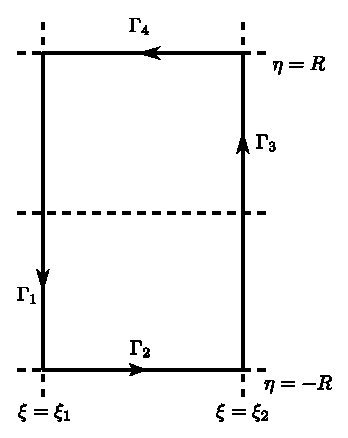
\includegraphics[scale=.9]{fig1.eps}
\end{figure}
where $\Gamma_1$ is the portion of the line $\xi = \xi_1$ lying
between the lines $\eta = \mathcal{R}$, $\eta = -\mathcal{R};
\Gamma_2$ is the portion of the line $\eta = -\mathcal{R}$ lying
between the lines $\xi = \xi_1$ and $\xi = \xi_2;\, \Gamma_3$ is the
line $\xi = \xi_2$ lying between the lines $\eta = -\mathcal{R}$ and
$\eta = \mathcal{R}$ and so on.

Now
$$
\lim_{R \to \infty}\int\limits_{\Gamma_2}|e^{pt} F(p)|\,|dp|=0 \quad
\text{and} \quad \lim_{R \to \infty} \int\limits_{\Gamma_4} |e^{pt}
F(p)|\,|dp|=0.
$$
Hence, we have $\quad \frac{1}{2\pi
  i}\left\{\int\limits_{\xi_1-i\infty}^{\xi +i\infty} e^{pt} F(p)\,dp +\quad
\int\limits_{\xi_2+i\infty}^{\xi_2-i\infty} e^{pt} F(p)\,dp \right\}=0$. 

\noindent In\pageoriginale other words, $f_{\xi_1}(t) - f_{\xi_2}
(t)=0$. Hence $f_{\xi_1}(t) = f_{\xi_2}(t)$. We now show that if $t <
0, f(t) = 0$, where $f(t)=f_\xi(t)$ for any $\xi \geq \xi_\circ
+\varepsilon$. In fact, $|f(t)|<\frac{A}{2}e^{\xi t}$. Allowing $\xi
\to \infty$ we have
$$
|f(t)| \leq 0.
$$
\begin{align*}
\text{Now, we have}\qquad f(t) &= \frac{1}{2\pi
  i}\int\limits_{-\infty}^\infty e^{\xi t}F(\xi + i \eta) e^{i\eta
  t}\; id\eta(\xi \geq \xi_\circ +\varepsilon)\\
&= \frac{1}{2\pi} e^{\xi t} \int\limits_{-\infty}^\infty F(\xi +
i\eta)e^{i\eta t}\,d\eta.
\end{align*}
Hence, $\quad 2 \pi e^{-\xi t} f(t) = \bar{\mathscr{F}_\eta}
(F(\xi+i\eta))$. Hence 
$$
F(\xi + i \eta) = \bar{\mathscr{F}_\eta}(e^{-\xi t}. 2\pi f(t) ).
$$
Hence $2 \pi e^{-\xi t} f(t)$ has for its $\eta$-Fourier transform the
function $F(\xi + i \eta)$, for any $\xi \geq \xi_\circ + \varepsilon, \varepsilon
>0$. Hence $f(t) \underset{\xi > \xi_\circ}{\sqsupset}F(p)$. Obviously
$f(t)$ defines a distribution in $\mathscr{D}_+'$ for $f(t)=0$, for
$t<0$.

Now suppose $F$ satisfies $|F(p)| \leq A(1 +|p|^2)^k$ in $\xi \geq
\xi_\circ + \varepsilon$ for any $\varepsilon > 0$, $k$ being an integer. The above is
equivalent to assuming 
$$
|F(p)| \leq A' |p|^{k'}
$$
where $k'$ is some integer and $A'$ is some constant, for $Rl p \geq
\xi_\circ + \varepsilon$. Now $\frac{F(p)}{p^{k'+2}}$ is holomorphic in $Rl p
> Max (0, \xi_\circ) = \nu$ (say), and for any $\varepsilon > 0$, we have
$$
\left|\frac{F(p)}{p^{k'+2}}\right|\leq\frac{A''}{(1+|p|^2)} \quad
\text{for} \quad Rl p \geq \nu + \varepsilon, 
$$
$A''$ being some constant. Hence by what we have proved, there exists
a distribution $T'\in \mathscr{D}_+'$ such that 
$$
T' \underset{\xi > \nu}{\sqsupset}\frac{F(p)}{p^{k'+2}}.
$$
Hence\pageoriginale $T = \underset{k'+2\text{ times}}{(\delta' *\cdots *\delta')}*
T'\underset{\xi>\nu}{\sqsupset}F(p)$, and $(\delta'*\cdots*\delta')* T'
\in \mathscr{D}_+'$. Thus we see that there exists a distribution
$T.\in \mathscr{D}_+'$ which has $F(p)$ as its Laplace transform in
the domain of definition of its Laplace transform.

That $T$ is unique follows from the fact that the Fourier transform
$\mathscr{F}:\mathscr{S}' \to \mathscr{S}'$ is an isomorphism onto.
